
\documentclass[10pt,a4paper]{article}
\usepackage[utf8]{inputenc}
\usepackage[portuguese]{babel}
\usepackage[margin=2cm]{geometry}
\usepackage{multicol}
\usepackage{enumitem}
\usepackage{xcolor}
\usepackage{listings}
\usepackage[box]{automultiplechoice}

% Configuração básica para exibição de códigos
\lstset{
  basicstyle=\small\ttfamily,
  breaklines=true
}

\begin{document}

{
\def\AMCbeginQuestion#1#2{\par\noindent{\bf (POSCOMP 2004 - Questão 68)}}
\begin{question}{} O protocolo padrão para gerenciamento de redes TCP/IP, definido pelo IETF, é:
\begin{choices}
\correctchoice{SNMP}
\wrongchoice{SMTP}
\wrongchoice{HTTP}
\wrongchoice{COPS}
\wrongchoice{SSH}
\end{choices}
\end{question}
}
%
{
\def\AMCbeginQuestion#1#2{\par\noindent{\bf (POSCOMP 2004 - Questão 69)}}
\begin{question}{} Qual das opções abaixo melhor caracteriza o protocolo IP?
\begin{choices}
\correctchoice{Não orientado a conexão, sem suporte a QoS, sem mecanismo de retransmissão.}
\wrongchoice{Orientado a conexão, com suporte a QoS, com mecanismo de retransmissão.}
\wrongchoice{Orientado a conexão, sem suporte a QoS, sem mecanismo de retransmissão.}
\wrongchoice{Orientado a conexão, sem suporte a QoS, com mecanismo de retransmissão.}
\wrongchoice{Não orientado a conexão, com suporte a QoS, sem mecanismo de retransmissão.}
\end{choices}
\end{question}
}
%
{
\def\AMCbeginQuestion#1#2{\par\noindent{\bf (POSCOMP 2004 - Questão 70)}}
\begin{question}{} Assinale a alternativa que apresenta um protocolo de roteamento baseado no algoritmo vetor-distância e é classificado como IGP (\textit{Interior Gateway Protocol}):
\begin{choices}
\correctchoice{RIP}
\wrongchoice{OSPF}
\wrongchoice{ICMP}
\wrongchoice{BGP}
\wrongchoice{RSVP}
\end{choices}
\end{question}
}
%
{
\def\AMCbeginQuestion#1#2{\par\noindent{\bf (POSCOMP 2005 - Questão 63)}}
\begin{question}{} Os protocolos de transporte atribuem a cada serviço um identificador único, o qual é empregado para encaminhar uma requisição de um aplicativo cliente ao processo servidor correto. Nos protocolos de transporte TCP e UDP, como esse identificador se denomina?
\begin{choices}
\correctchoice{Porta.}
\wrongchoice{Endereço IP.}
\wrongchoice{Conexão.}
\wrongchoice{Identificador do processo (PID).}
\wrongchoice{Protocolo de aplicação.}
\end{choices}
\end{question}
}
%
{
\def\AMCbeginQuestion#1#2{\par\noindent{\bf (POSCOMP 2005 - Questão 64)}}
\begin{question}{} O DNS (\textit{Domain Name System}) é um serviço de diretórios na Internet que:
\begin{choices}
\correctchoice{Traduz o nome de um hospedeiro (host) para seu endereço IP.}
\wrongchoice{Localiza a instituição à qual um dado host pertence.}
\wrongchoice{Retorna a porta da conexão TCP do host.}
\wrongchoice{Retorna a porta da conexão UDP do host.}
\wrongchoice{Traduz o endereço IP de um hospedeiro para um nome de domínio na Internet.}
\end{choices}
\end{question}
}
%
{
\def\AMCbeginQuestion#1#2{\par\noindent{\bf (POSCOMP 2005 - Questão 65)}}
\begin{question}{} Um dos mecanismos de congestionamento na rede é o que utiliza temporizadores de transmissão e duas variáveis chamadas de: Janela de Congestionamento e Patamar. A Janela de Congestionamento impõe um limite à quantidade de tráfego que um host pode enviar dentro de uma conexão. O Patamar é uma variável que regula o crescimento da Janela de Congestionamento durante as transmissões daquela conexão. Assinale a alternativa correta:
\begin{choices}
\correctchoice{A Janela de Congestionamento dobra de tamanho (cresce exponencialmente) quando a confirmação das mensagens enviadas ocorre antes dos temporizadores de retransmissão se esgotarem (\textit{time-out}), até o limite do Patamar.}
\wrongchoice{A quantidade de mensagens não confirmadas na transmissão, num dado instante, deve ser superior ao mínimo entre a Janela de Congestionamento e a Janela de Recepção desta conexão.}
\wrongchoice{Após exceder o valor de Patamar ainda sem esgotar os temporizadores, a janela decresce linearmente.}
\wrongchoice{Quando excede o valor de Patamar e esgotam os temporizadores, a janela decresce exponencialmente.}
\wrongchoice{Todas as alternativas estão corretas.}
\end{choices}
\end{question}
}
%
{
\def\AMCbeginQuestion#1#2{\par\noindent{\bf (POSCOMP 2005 - Questão 66)}}
\begin{question}{} Algoritmos de roteamento são o meio que um roteador utiliza para encaminhar mensagens na camada de rede. Assinale a alternativa incorreta.
\begin{choices}
\correctchoice{No roteamento de Estado de Enlace (\textit{Link State}), os valores dos enlaces são calculados pelo projetista da rede e os roteadores atualizam suas tabelas por estes valores.}
\wrongchoice{Nos algoritmos de roteamento estáticos as rotas são determinadas via tabelas definidas a priori e fixadas para o roteador, em geral manualmente.}
\wrongchoice{No roteamento por Vetor de Distância (\textit{Distance Vector}), as tabelas de roteamento definidas pelos roteadores vizinhos são repassadas periodicamente a cada roteador para obtenção de sua própria tabela.}
\wrongchoice{Algoritmos de roteamento buscam estabelecer o caminho de menor custo entre dois hosts através do cálculo dos custos acumulados mínimos entre os enlaces disponíveis, dada a topologia da rede.}
\wrongchoice{O OSPF é um exemplo de protocolo de roteamento baseado em Estado de Enlace e o BGP é um exemplo de protocolo de roteamento baseado em Vetor de Distâncias.}
\end{choices}
\end{question}
}
%
{
\def\AMCbeginQuestion#1#2{\par\noindent{\bf (POSCOMP 2005 - Questão 67)}}
\begin{question}{} Sejam as afirmações:
\begin{enumerate}[label=\Roman*.]
\item O HTTP e o FTP são protocolos da camada de aplicação e utilizam o protocolo de transporte TCP.
\item Ambos (HTTP e FTP) utilizam duas conexões TCP, uma para controle da transferência e outra para envio dos dados transferidos (controle fora da banda).
\item O HTTP pode usar conexões não persistentes e persistentes. O HTTP/1.0 usa conexões não persistentes. O modo default do HTTP/1.1 usa conexões persistentes.
\end{enumerate}
Dadas estas três afirmações, indique qual a alternativa correta:
\begin{choices}
\correctchoice{Somente I e III são verdadeiras.}
\wrongchoice{I, II e III são verdadeiras.}
\wrongchoice{Somente I e II são verdadeiras.}
\wrongchoice{Somente I é verdadeira.}
\wrongchoice{I, II e III são falsas.}
\end{choices}
\end{question}
}
%
{
\def\AMCbeginQuestion#1#2{\par\noindent{\bf (POSCOMP 2006 - Questão 64)}}
\begin{question}{} Sobre o protocolo IP (\textit{Internet Protocol}), é correto afirmar:
\begin{choices}
\correctchoice{O espaço de endereçamento do IPv4 e do IPv6 é de 32 e 128 bits, respectivamente.}
\wrongchoice{O tamanho do cabeçalho do IPv4 é fixado em 96 bits.}
\wrongchoice{O cabeçalho IP inclui informação sobre o protocolo de camada de enlace empregado.}
\wrongchoice{A classe C de endereços IPv4 reserva 16 bits para endereço de rede.}
\wrongchoice{O roteamento IP associa o endereço IP com o número de porta em nível de transporte.}
\end{choices}
\end{question}
}
%
{
\def\AMCbeginQuestion#1#2{\par\noindent{\bf (POSCOMP 2006 - Questão 65)}}
\begin{question}{} Duas tecnologias utilizadas para acesso residencial à Internet são ADSL e Cable Modem. Qual afirmação é incorreta?
\begin{choices}
\correctchoice{Os canais de \textit{upstream} e \textit{downstream} da tecnologia Cable Modem necessitam de contenção de acesso.}
\wrongchoice{Ambas permitem taxas de transmissão diferentes para \textit{upstream} e \textit{downstream}.}
\wrongchoice{Os canais de \textit{upstream} e \textit{downstream} da tecnologia ADSL não necessitam de contenção de acesso.}
\wrongchoice{ADSL utiliza par trançado dedicado para cada residência.}
\wrongchoice{Cable Modem utiliza cabo compartilhado para diversas residências.}
\end{choices}
\end{question}
}
%
{
\def\AMCbeginQuestion#1#2{\par\noindent{\bf (POSCOMP 2006 - Questão 66)}}
\begin{question}{} Os endereços IP são divididos em classes. Qual afirmação é incorreta?
\begin{choices}
\correctchoice{Máscaras podem dividir o campo Rede do endereço IP em Rede e Sub-rede para facilitar o roteamento interno.}
\wrongchoice{Existem mais redes classe B do que classe A.}
\wrongchoice{Uma rede classe C permite mais hosts do que uma rede classe B.}
\wrongchoice{A classe D é dedicada a endereços \textit{multicast}.}
\wrongchoice{NAT (Tradução de Endereço de Rede) é utilizada em redes com vários hosts que se conectam à Internet através de poucos endereços IP.}
\end{choices}
\end{question}
}
%
{
\def\AMCbeginQuestion#1#2{\par\noindent{\bf (POSCOMP 2007 - Questão 64)}}
\begin{question}{} O controle de congestionamento é uma das funções desempenhadas pela Camada de Transporte no modelo TCP/IP. Sobre essa função, assinale a alternativa INCORRETA.
\begin{choices}
\correctchoice{No controle de congestionamento assistido pela rede, os nodos (roteadores) enviam notificações explícitas do estado de congestionamento da rede diretamente à fonte de cada fluxo que, por meio dele, trafega.}
\wrongchoice{No controle de congestionamento fim-a-fim, uma situação de congestionamento é intuída pelos hosts terminais via eventos como perda ou atraso excessivo de pacotes.}
\wrongchoice{O mecanismo \textit{Explicit Congestion Notification} (ECN) utiliza um dos dois últimos bits do campo ToS do cabeçalho IPv4 para notificar a um destinatário o estado de congestionamento da rede.}
\wrongchoice{Ao perceber um estado de congestionamento na rede, uma conexão TCP, por meio de seu mecanismo de prevenção de congestionamento (\textit{congestion avoidance}), reduz o tamanho de sua janela de congestionamento.}
\wrongchoice{Na fase de partida lenta (\textit{slow start}) de uma conexão TCP, o tamanho da janela de congestionamento aumenta a cada RTT (\textit{Round-Trip Time}) de forma exponencial, até que esse tamanho alcance um determinado valor de limiar (\textit{threshold}).}
\end{choices}
\end{question}
}
%
{
\def\AMCbeginQuestion#1#2{\par\noindent{\bf (POSCOMP 2007 - Questão 65)}}
\begin{question}{} Sobre o protocolo de transferência de hipertextos (HTTP - \textit{Hyper-Text Transfer Protocol}), é CORRETO afirmar que
\begin{choices}
\correctchoice{A instrução GET condicional permite que o cliente opte por receber um determinado objeto do servidor apenas se este tiver sido alterado depois de uma determinada data e hora.}
\wrongchoice{O protocolo HTTP é capaz de transportar nativamente arquivos no formato binário.}
\wrongchoice{A versão 1.0 do protocolo HTTP não permite a utilização de cookies.}
\wrongchoice{A versão 1.1 do protocolo HTTP difere da versão 1.0 na capacidade de transportar objetos maiores.}
\wrongchoice{O protocolo HTTP não pode ser utilizado para transportar outros tipos de objetos senão os hiper-textos.}
\end{choices}
\end{question}
}
%
{
\def\AMCbeginQuestion#1#2{\par\noindent{\bf (POSCOMP 2007 - Questão 66)}}
\begin{question}{} Considere os pares de endereços de hosts e suas respectivas máscaras de endereços listados abaixo.
\begin{enumerate}[label=\Roman*.]
\item 192.168.0.43/255.255.255.192 e 192.168.0.66/255.255.255.192
\item 192.168.1.97/255.255.255.224 e 192.168.1.118/255.255.255.224
\item 192.168.2.115/255.255.255.128 e 192.168.2.135/255.255.255.128
\item 192.168.3.34/255.255.255.240 e 192.168.3.46/255.255.255.240
\item 192.168.4.167/255.255.255.224 e 192.168.4.207/255.255.255.224
\end{enumerate}
Os itens nos quais o par citado pertence a uma mesma sub-rede são
\begin{choices}
\correctchoice{apenas II, IV.}
\wrongchoice{apenas I, II, V.}
\wrongchoice{apenas I, III.}
\wrongchoice{apenas II, III, IV.}
\wrongchoice{apenas III, IV, V.}
\end{choices}
\end{question}
}
%
{
\def\AMCbeginQuestion#1#2{\par\noindent{\bf (POSCOMP 2007 - Questão 67)}}
\begin{question}{} Analise as seguintes afirmativas.
\begin{enumerate}[label=\Roman*.]
\item O protocolo UDP é um protocolo da Camada de Transporte orientado a datagrama, enquanto que o TCP é um protocolo da Camada de Transporte orientado a conexão.
\item Apesar de o protocolo IP ser orientado a datagrama, o protocolo UDP é necessário por fornecer multiplexação de um endereço de rede em várias portas, permitindo que múltiplos processos sejam endereçados em um mesmo endereço de rede.
\item O protocolo TCP utiliza o tamanho da janela deslizante de uma conexão para o controle de congestionamento.
\end{enumerate}
A esse respeito, pode-se afirmar que
\begin{choices}
\correctchoice{todas as afirmativas são corretas.}
\wrongchoice{somente a afirmativa I é correta.}
\wrongchoice{somente as afirmativas I e II são corretas.}
\wrongchoice{somente as afirmativas I e III são corretas.}
\wrongchoice{somente as afirmativas II e III são corretas.}
\end{choices}
\end{question}
}
%
{
\def\AMCbeginQuestion#1#2{\par\noindent{\bf (POSCOMP 2008 - Questão 07)}}
\begin{question}{} Analise as seguintes afirmativas.
\begin{enumerate}[label=\Roman*.]
\item Um servidor DNS suporta dois tipos de consulta: iterativa e recursiva. Na consulta iterativa que é a mais utilizada, caso um servidor DNS não tenha a informação pedida pela máquina solicitante, ele irá buscar a mesma consultando outros servidores.
\item Como estratégia para aumentar a confiabilidade na resposta dos servidores DNS quando do emprego de caches, devem-se utilizar valores grandes de TLL (\textit{Time-To-Live}), mantendo elevado o tempo de validade do registro na cache.
\item Um servidor DNS pode atender dois tipos de consultas: tradução direta, na qual, a partir de um endereço IP, o mesmo retorna o nome de rede do equipamento; e tradução inversa, na qual, a partir de um nome de rede, retorna o IP associado ao mesmo.
\end{enumerate}
A análise permite concluir que
\begin{choices}
\correctchoice{nenhuma afirmativa está correta.}
\wrongchoice{somente a afirmativa I está correta.}
\wrongchoice{somente a afirmativa II está correta.}
\wrongchoice{somente a afirmativa III está correta.}
\wrongchoice{todas as afirmativas estão corretas.}
\end{choices}
\end{question}
}
%
{
\def\AMCbeginQuestion#1#2{\par\noindent{\bf (POSCOMP 2008 - Questão 08)}}
\begin{question}{} O nível de transporte oferece serviços para comunicação entre computadores, independentemente das tecnologias utilizadas nos outros níveis.

Analise as seguintes afirmativas relativas à confirmação do recebimento de pacotes no nível de transporte.
\begin{enumerate}[label=\Roman*.]
\item A troca de dados entre um computador transmissor e um receptor não precisa obrigatoriamente de uma confirmação para cada pacote enviado. Existem três estratégias que podem ser utilizadas: confirmação seletiva, confirmação cumulativa e confirmação em bloco.
\item Na confirmação seletiva, cada pacote recebido por um computador não gera uma informação de confirmação individualizada para o computador que enviou o pacote.
\item Na confirmação do recebimento de pacotes, o consumo da banda de rede pode ser otimizado pelo uso de um mecanismo denominado \textit{piggybacking}. No \textit{piggybacking} a informação de confirmação ``pega carona'' em mensagem de dados que retorna ao computador emissor como consequência do fluxo normal de troca de dados.
\end{enumerate}
A análise permite concluir que
\begin{choices}
\correctchoice{apenas as afirmativas I e III estão corretas.}
\wrongchoice{nenhuma das afirmativas está correta.}
\wrongchoice{apenas as afirmativas I e II estão corretas.}
\wrongchoice{apenas as afirmativas II e III estão corretas.}
\wrongchoice{todas as afirmativas estão corretas.}
\end{choices}
\end{question}
}
%
{
\def\AMCbeginQuestion#1#2{\par\noindent{\bf (POSCOMP 2008 - Questão 14)}}
\begin{question}{} Sobre a comunicação entre processos distribuídos, é CORRETO afirmar
\begin{choices}
\correctchoice{que, nos sockets do tipo datagrama, o endereço do socket do processo correspondente acompanha cada envio de mensagem como um parâmetro da primitiva \texttt{sendto()}.}
\wrongchoice{que, no modo síncrono de envio de mensagem, o processo que recebe a mensagem terá sua execução desviada por uma interrupção de sistema operacional para tratar uma mensagem recebida.}
\wrongchoice{que um processo tem no máximo uma porta (port) para receber as mensagens dos seus interlocutores.}
\wrongchoice{que multiportas são estruturas do tipo portas multicast que permitem a comunicação N x M entre processos.}
\wrongchoice{que, nos sockets do tipo datagrama, a primitiva \texttt{sNew()} é usada para aceitar a conexão solicitada por um processo que solicita comunicação.}
\end{choices}
\end{question}
}
%
{
\def\AMCbeginQuestion#1#2{\par\noindent{\bf (POSCOMP 2009 - Questão 62)}}
\begin{question}{} Os mecanismos de controle de congestionamento e controle de fluxo desempenham um papel fundamental no projeto de uma rede de computadores. Considere as afirmativas a seguir sobre os dois mecanismos.
\begin{enumerate}[label=\Roman*.]
\item O mecanismo de controle de congestionamento regula (ou seja, aumenta e diminui dinamicamente) a taxa com a qual o transmissor envia dados pela rede.
\item O mecanismo de controle de congestionamento garante que o receptor irá receber todos os dados enviados pelo transmissor.
\item O mecanismo de controle de fluxo regula (ou seja, aumenta e diminui dinamicamente) a taxa com a qual o transmissor envia dados pela rede.
\item O mecanismo de controle de fluxo garante que o receptor irá receber todos os dados enviados pelo transmissor.
\end{enumerate}
Assinale a alternativa CORRETA:
\begin{choices}
\correctchoice{Apenas as alternativas I e III são verdadeiras.}
\wrongchoice{Apenas as alternativas I, II e III são verdadeiras.}
\wrongchoice{Apenas as alternativas II e IV são verdadeiras.}
\wrongchoice{Apenas as alternativas III e IV são verdadeiras.}
\wrongchoice{Todas as alternativas são verdadeiras.}
\end{choices}
\end{question}
}
%
{
\def\AMCbeginQuestion#1#2{\par\noindent{\bf (POSCOMP 2009 - Questão 63)}}
\begin{question}{} Um dos problemas importantes na Internet é o endereçamento de processos, ou seja, aplicações em execução em um determinado computador.

Considere as afirmativas a seguir.
\begin{enumerate}[label=\Roman*.]
\item Todo pacote transmitido precisa conter o endereço IP e a porta do processo destino.
\item Pacotes do protocolo TCP não precisam conter o endereço IP nem a porta do processo do transmissor.
\item A tupla endereço IP de origem e destino e porta de origem e destino identificam unicamente uma conexão TCP.
\item Um processo que utiliza o protocolo UDP para se comunicar nunca recebe pacotes fora da ordem em que foram transmitidos.
\end{enumerate}
Assinale a alternativa CORRETA:
\begin{choices}
\correctchoice{Apenas as alternativas I e III são verdadeiras.}
\wrongchoice{Apenas as alternativas I e II são verdadeiras.}
\wrongchoice{Apenas as alternativas II e III são verdadeiras.}
\wrongchoice{Apenas as alternativas I, III e IV são verdadeiras.}
\wrongchoice{Todas as alternativas são verdadeiras.}
\end{choices}
\end{question}
}
%
{
\def\AMCbeginQuestion#1#2{\par\noindent{\bf (POSCOMP 2010 - Questão 56)}}
\begin{question}{} Em uma rede de computadores, cujos roteadores estão configurados para atualizar suas tabelas de roteamento por meio do emprego de protocolos de roteamento, é correto afirmar:
\begin{choices}
\correctchoice{Roteadores de borda, que ligam a rede local a redes remotas, tipicamente suportam dois protocolos de roteamento: um protocolo interno para a comunicação com os roteadores locais e um protocolo externo para a comunicação com os roteadores de redes remotas.}
\wrongchoice{Ao se interromper o uso dos protocolos de roteamento, a rede deixará de operar porque não haverá possibilidade de atualização das tabelas de roteamento dos roteadores.}
\wrongchoice{Roteadores que empregam protocolos de roteamento trocam mensagens de controle de tais protocolos apenas quando os enlaces da rede se tornam inoperantes ou quando os mesmos voltam a operar.}
\wrongchoice{O RIP (\textit{Routing Information Protocol}), que emprega o algoritmo de roteamento vetor distância, vem sucedendo nas redes locais o protocolo OSPF (\textit{Open Shortest Path First}), o qual emprega o algoritmo estado de enlace.}
\wrongchoice{Protocolos de aplicação, como o HTTP, podem diretamente controlar os protocolos de roteamento ao solicitarem que os roteadores da rede calculem rotas alternativas para transportar o tráfego dos protocolos de aplicação.}
\end{choices}
\end{question}
}
%
{
\def\AMCbeginQuestion#1#2{\par\noindent{\bf (POSCOMP 2010 - Questão 58)}}
\begin{question}{} O SNMP (\textit{Simple Network Management Protocol}) é o mais difundido protocolo de gerenciamento de redes TCP/IP. Sobre o SNMP, é correto afirmar:
\begin{choices}
\correctchoice{A mensagem \texttt{GetBulkRequest} permite a recuperação de várias instâncias de um mesmo objeto.}
\wrongchoice{A versão 1 do SNMP, apesar de empregar mensagens criptografadas, não possui mecanismo de autenticação de mensagens junto aos dispositivos gerenciados.}
\wrongchoice{A mensagem \texttt{SetRequest} é utilizada tanto para alterar quanto para ler o valor das instâncias dos objetos gerenciados.}
\wrongchoice{A configuração de dispositivos de rede por meio do SNMP é mais aceita que a monitoração de redes pelo SNMP.}
\wrongchoice{Mensagens \textit{trap} são utilizadas por gerentes SNMP para notificar agentes SNMP sobre as modificações internas do sistema de gerenciamento.}
\end{choices}
\end{question}
}
%
{
\def\AMCbeginQuestion#1#2{\par\noindent{\bf (POSCOMP 2011 - Questão 64)}}
\begin{question}{} Em relação à transmissão com fibras óticas, considere as afirmativas a seguir.
\begin{enumerate}[label=\Roman*.]
\item A velocidade de propagação em uma fibra ótica é muito superior à velocidade de propagação em um cabo coaxial.
\item Uma fibra monomodo, por permitir à luz se propagar apenas em um modo, permite obter uma taxa em bps bem superior à de uma fibra multimodo.
\item Pode-se ter comunicação \textit{full-duplex} (transmissão simultânea nos dois sentidos) utilizando-se apenas uma fibra única e não um par de fibras.
\item A atenuação em fibra ótica ocorre devido principalmente à absorção (produção de calor) e radiação e independe do comprimento de onda utilizado na transmissão da luz.
\end{enumerate}
Assinale a alternativa correta.
\begin{choices}
\correctchoice{Somente as afirmativas II e III são corretas.}
\wrongchoice{Somente as afirmativas I e IV são corretas.}
\wrongchoice{Somente as afirmativas III e IV são corretas.}
\wrongchoice{Somente as afirmativas I, II e III são corretas.}
\wrongchoice{Somente as afirmativas I, II e IV são corretas.}
\end{choices}
\end{question}
}
%
{
\def\AMCbeginQuestion#1#2{\par\noindent{\bf (POSCOMP 2011 - Questão 65)}}
\begin{question}{} Com base na divisão dos protocolos de comunicação em camadas, assinale a alternativa correta.
\begin{choices}
\correctchoice{Uma camada pode oferecer um serviço confiável para uma camada acima, mesmo que a camada abaixo não seja confiável.}
\wrongchoice{O modelo de protocolos em camadas define que protocolos são utilizados entre as camadas de um mesmo hospedeiro.}
\wrongchoice{No modelo em camadas, cada camada suporta apenas um único protocolo.}
\wrongchoice{O uso de camadas em protocolos de comunicação surgiu para diminuir o \textit{overhead}.}
\wrongchoice{A arquitetura TCP/IP padroniza os protocolos das camadas física e de enlace.}
\end{choices}
\end{question}
}
%
{
\def\AMCbeginQuestion#1#2{\par\noindent{\bf (POSCOMP 2011 - Questão 67)}}
\begin{question}{} Assuma uma topologia de rede local Ethernet comutada, formada pela interconexão de três comutadores (\textit{switches} SW1, SW2 e SW3), como mostrado a seguir.
\begin{center}
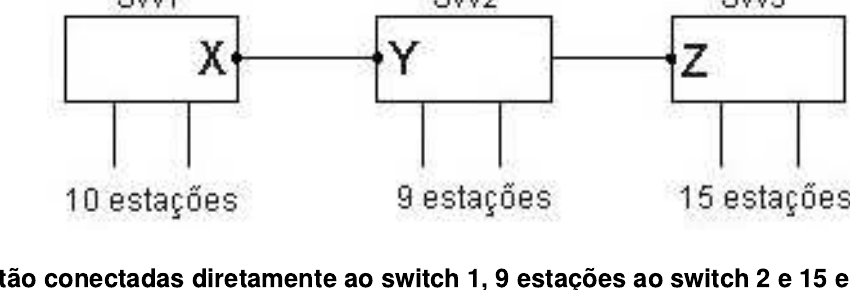
\includegraphics[width=0.55\textwidth]{poscomp_2011_q67_figura.png}
\end{center}
10 estações estão conectadas diretamente ao switch 1, 9 estações ao switch 2 e 15 estações ao switch 3. Supondo-se que todas as estações estão ativas e transmitindo na rede local simultaneamente, assinale a alternativa correta quanto à quantidade mínima de endereços MAC a serem armazenados nos buffers das portas X (de SW1), Y (de SW2) e Z (de SW3) para que não haja a necessidade de geração de broadcast numa transmissão entre duas estações quaisquer, após o equilíbrio no preenchimento dos buffers para armazenamento de endereço MAC nas portas dos comutadores.
\begin{choices}
\correctchoice{X=24, Y=10, Z=19}
\wrongchoice{X=10, Y=9, Z=15}
\wrongchoice{X=9, Y=10, Z=15}
\wrongchoice{X=34, Y=34, Z=34}
\wrongchoice{X=10, Y=25, Z=15}
\end{choices}
\end{question}
}
%
{
\def\AMCbeginQuestion#1#2{\par\noindent{\bf (POSCOMP 2011 - Questão 69)}}
\begin{question}{} Sobre o acesso residencial de banda larga, através de modem a cabo (\textit{cable modem}) ou ADSL (\textit{asymmetrical digital subscriber line}), assinale a afirmativa correta.
\begin{choices}
\correctchoice{Na tecnologia de modem a cabo, a taxa máxima de transmissão (em bps) é variável e alocada de acordo com a demanda do usuário.}
\wrongchoice{O desempenho do acesso em arquitetura de modem a cabo independe de quantos usuários estão usando simultaneamente a rede, porque o cabo trabalha com multiplexação em frequência (FDM).}
\wrongchoice{A banda passante usada nas comunicações digitais através das linhas de assinante, como visto na tecnologia ADSL, é a mesma usada para a transmissão de voz e é da ordem de 4 kHz.}
\wrongchoice{Em ADSL, a taxa máxima de operação em bps independe do nível de ruído da linha e da distância até a central da operadora.}
\wrongchoice{Em ADSL, trabalha-se com multiplexação em frequência, e a taxa de acesso do assinante depende do acesso de outros usuários.}
\end{choices}
\end{question}
}
%
{
\def\AMCbeginQuestion#1#2{\par\noindent{\bf (POSCOMP 2012 - Questão 60)}}
\begin{question}{} O modelo de referência OSI (\textit{Open Systems Interconnection}) é composto por 7 camadas. Sobre as funções destas camadas, assinale a alternativa correta.
\begin{choices}
\correctchoice{A camada de apresentação realiza conversões para permitir a interação entre computadores com diferentes representações de dados.}
\wrongchoice{A camada física delimita quadros e realiza controle de fluxo antes de entregar os dados para as camadas superiores.}
\wrongchoice{A camada de transporte define a rota de menor custo que os pacotes percorrerão no percurso entre o transmissor e o receptor.}
\wrongchoice{A camada de sessão é responsável pelo endereçamento dos pacotes que serão transmitidos durante a vigência de uma sessão.}
\wrongchoice{Na hierarquia de camadas do modelo OSI, a camada de rede se posiciona entre a camada de transporte e a camada de sessão.}
\end{choices}
\end{question}
}
%
{
\def\AMCbeginQuestion#1#2{\par\noindent{\bf (POSCOMP 2012 - Questão 62)}}
\begin{question}{} O TCP (\textit{Transport Control Protocol}) é um protocolo da camada de transporte da arquitetura TCP/IP. Sobre o TCP, assinale a alternativa correta.
\begin{choices}
\correctchoice{O algoritmo \textit{three way handshake} (apresentação de três vias) é utilizado para estabelecer uma conexão lógica entre transmissor e receptor.}
\wrongchoice{Ao estabelecer uma conexão lógica entre o transmissor e o receptor, o TCP realiza reserva de banda para garantir qualidade de serviço.}
\wrongchoice{O algoritmo de controle de congestionamento verifica o estado dos buffers de cada roteador presente no caminho entre o transmissor e o receptor.}
\wrongchoice{O TCP é utilizado em aplicações de tempo real e sensíveis à latência que necessitam de agilidade na transmissão e dispensam a confiabilidade.}
\wrongchoice{Por realizar controle de fluxo, o TCP não contém vulnerabilidades que podem ser exploradas em ataques de negação de serviço.}
\end{choices}
\end{question}
}
%
{
\def\AMCbeginQuestion#1#2{\par\noindent{\bf (POSCOMP 2012 - Questão 66)}}
\begin{question}{} Os padrões IEEE 802.11 são amplamente utilizados para a construção de redes locais sem fio. Sobre esses padrões, assinale a alternativa correta.
\begin{choices}
\correctchoice{Um dos diferenciais do padrão IEEE 802.11n com relação a seus antecessores é a adoção da tecnologia MIMO (\textit{Multiple Input Multiple Output}).}
\wrongchoice{O protocolo de segurança WEP (\textit{Wired Equivalent Privacy}) é recomendado para as redes IEEE 802.11 por não ter vulnerabilidades conhecidas.}
\wrongchoice{O protocolo de acesso ao meio utilizado nas redes IEEE 802.11 é o mesmo utilizado pelas redes Ethernet e se baseia na detecção de colisão.}
\wrongchoice{O IEEE 802.11 é uma das principais tecnologias da quarta geração (4G) de sistemas para telefonia celular, juntamente com o IEEE 802.16.}
\wrongchoice{O padrão IEEE 802.11b foi bastante adotado por proporcionar taxas de transmissão de 1 gigabit por segundo a distâncias de até 50 m.}
\end{choices}
\end{question}
}
%
{
\def\AMCbeginQuestion#1#2{\par\noindent{\bf (POSCOMP 2013 - Questão 61)}}
\begin{question}{} Com relação aos meios físicos de transmissão utilizados em redes de comunicação, considere as afirmativas a seguir.
\begin{enumerate}[label=\Roman*.]
\item As fibras óticas monomodo apresentam uma atenuação maior que as fibras multimodo e são mais baratas.
\item Nos cabos de par trançado, a largura de banda disponível é independente da distância percorrida pelo cabeamento.
\item Nas transmissões em fibras óticas, a fonte de luz pode ser um LED (\textit{Light Emitting Diode}) ou um laser semicondutor.
\item Os cabos coaxiais, em suas versões mais modernas, podem apresentar largura de banda da ordem de GHz.
\end{enumerate}
Assinale a alternativa correta.
\begin{choices}
\correctchoice{Somente as afirmativas III e IV são corretas.}
\wrongchoice{Somente as afirmativas I e II são corretas.}
\wrongchoice{Somente as afirmativas I e IV são corretas.}
\wrongchoice{Somente as afirmativas I, II e III são corretas.}
\wrongchoice{Somente as afirmativas II, III e IV são corretas.}
\end{choices}
\end{question}
}
%
{
\def\AMCbeginQuestion#1#2{\par\noindent{\bf (POSCOMP 2013 - Questão 63)}}
\begin{question}{} Sobre o IPSec, assinale a alternativa correta.
\begin{choices}
\correctchoice{A utilização do IPSec depende do estabelecimento de uma SA (\textit{Security Association}).}
\wrongchoice{No IPv6, os dados do IPSec são transportados pelo cabeçalho IP principal.}
\wrongchoice{O IPSec é incompatível com o IPv4, mas pode ser utilizado com o IPv6.}
\wrongchoice{É impossível construir \textit{Virtual Private Networks} (VPN) utilizando o IPSec.}
\wrongchoice{Um grave problema do IPSec é a ausência de soluções de autenticação.}
\end{choices}
\end{question}
}
%
{
\def\AMCbeginQuestion#1#2{\par\noindent{\bf (POSCOMP 2013 - Questão 65)}}
\begin{question}{} A arquitetura TCP/IP inclui protocolos de aplicação que fornecem importantes serviços como FTP, SMTP, SNMP, DNS e HTTP.

Com relação aos protocolos de aplicação da arquitetura TCP/IP, atribua V (verdadeiro) ou F (falso) às afirmativas a seguir.
\begin{itemize}[label={(\ )}]
\item O FTP usa duas conexões paralelas para transferir arquivos: uma conexão de controle e uma conexão de dados.
\item O SMTP transfere mensagens do servidor de e-mail do remetente para o servidor de e-mail do destinatário.
\item O SNMP utiliza o protocolo de transporte TCP, pois não tolera as perdas de dados que podem ocorrer com o UDP.
\item O DNS é organizado de forma distribuída e hierárquica para proporcionar escalabilidade na resolução de nomes.
\item No HTTP, o método INVITE é utilizado para que o cliente comunique ao servidor que deseja estabelecer uma sessão.
\end{itemize}
Assinale a alternativa que contém, de cima para baixo, a sequência correta.
\begin{choices}
\correctchoice{V, V, F, V, F.}
\wrongchoice{V, F, V, F, F.}
\wrongchoice{F, V, V, V, F.}
\wrongchoice{F, V, F, V, V.}
\wrongchoice{F, F, V, F, V.}
\end{choices}
\end{question}
}
%
{
\def\AMCbeginQuestion#1#2{\par\noindent{\bf (POSCOMP 2014 - Questão 54)}}
\begin{question}{} Suponha que o administrador de uma rede está utilizando o seguinte prefixo para uma de suas sub-redes: 128.208.0.64/26. Assinale a alternativa que apresenta, corretamente, um endereço IP pertencente a essa sub-rede.
\begin{choices}
\correctchoice{128.208.0.122}
\wrongchoice{128.208.0.56}
\wrongchoice{128.208.0.160}
\wrongchoice{128.208.0.200}
\wrongchoice{128.208.0.225}
\end{choices}
\end{question}
}
%
{
\def\AMCbeginQuestion#1#2{\par\noindent{\bf (POSCOMP 2014 - Questão 60)}}
\begin{question}{} O modelo de referência Open Systems Interconnection (OSI) é dividido em sete camadas. Cada uma dessas camadas tem suas respectivas tarefas. Uma das tarefas previstas no modelo OSI é a de transformar um canal de transmissão físico em uma linha que pareça livre de erros de transmissão. Assinale a alternativa que apresenta, corretamente, a camada responsável por essa tarefa.
\begin{choices}
\correctchoice{Camada de enlace de dados.}
\wrongchoice{Camada de aplicação.}
\wrongchoice{Camada de apresentação.}
\wrongchoice{Camada de rede.}
\wrongchoice{Camada de sessão.}
\end{choices}
\end{question}
}
%
{
\def\AMCbeginQuestion#1#2{\par\noindent{\bf (POSCOMP 2014 - Questão 65)}}
\begin{question}{} Os padrões Ethernet englobam diferentes meios físicos de transmissão, diversas distâncias máximas de segmento e várias velocidades de transmissão. Com base nos conhecimentos sobre o tema, assinale a alternativa que apresenta, corretamente, um padrão Ethernet que utiliza a fibra óptica como meio de transmissão, permite distâncias máximas de segmento superiores a 15 km e oferece velocidades de transmissão iguais ou superiores a 10 Gbps.
\begin{choices}
\correctchoice{10GBASE-ER}
\wrongchoice{10GBASE-SR}
\wrongchoice{10GBASE-T}
\wrongchoice{100BASE-FX}
\wrongchoice{1000BASE-T}
\end{choices}
\end{question}
}
%
{
\def\AMCbeginQuestion#1#2{\par\noindent{\bf (POSCOMP 2015 - Questão 54)}}
\begin{question}{} Normalmente, existem vários caminhos entre origem e destino em uma rede de computadores. O processo de descobrir um caminho que funcione por meio de uma rede é denominado
\begin{choices}
\correctchoice{roteamento.}
\wrongchoice{encaminhamento.}
\wrongchoice{nomeação.}
\wrongchoice{descobrimento.}
\wrongchoice{endereçamento.}
\end{choices}
\end{question}
}
%
{
\def\AMCbeginQuestion#1#2{\par\noindent{\bf (POSCOMP 2015 - Questão 60)}}
\begin{question}{} Na transmissão de dados, quando um transmissor rápido enviar uma quantidade excessiva de dados a um receptor mais lento, deve-se aplicar
\begin{choices}
\correctchoice{o controle de fluxo.}
\wrongchoice{o controle de congestionamento.}
\wrongchoice{a retroalimentação.}
\wrongchoice{a adaptação.}
\wrongchoice{a transferência.}
\end{choices}
\end{question}
}
%
{
\def\AMCbeginQuestion#1#2{\par\noindent{\bf (POSCOMP 2015 - Questão 65)}}
\begin{question}{} No modelo de referência ISO/OSI, qual camada deve gerenciar tokens, impedindo que duas partes tentem executar, ao mesmo tempo, a mesma operação crítica?
\begin{choices}
\correctchoice{Sessão}
\wrongchoice{Transporte}
\wrongchoice{Apresentação}
\wrongchoice{Sincronização}
\wrongchoice{Aplicação}
\end{choices}
\end{question}
}
%
{
\def\AMCbeginQuestion#1#2{\par\noindent{\bf (POSCOMP 2016 - Questão 60)}}
\begin{question}{} Em relação às características do protocolo IP, analise as afirmativas abaixo e assinale V, se verdadeiras, ou F, se falsas.
\begin{itemize}[label={(\ )}]
\item O protocolo IP garante a entrega de mensagens.
\item O endereçamento IP é hierárquico.
\item O protocolo IP garante que não há duplicação de pacotes.
\end{itemize}
A ordem correta de preenchimento dos parênteses, de cima para baixo, é:
\begin{choices}
\correctchoice{F – V – F.}
\wrongchoice{F – F – V.}
\wrongchoice{V – F – V.}
\wrongchoice{V – V – F.}
\wrongchoice{V – F – F.}
\end{choices}
\end{question}
}
%
{
\def\AMCbeginQuestion#1#2{\par\noindent{\bf (POSCOMP 2016 - Questão 65)}}
\begin{question}{} Uma rede conectada a Internet possui a máscara de sub-rede 255.255.255.0. Qual o número máximo de computadores que a rede suporta?
\begin{choices}
\correctchoice{254.}
\wrongchoice{224.}
\wrongchoice{128.}
\wrongchoice{65534.}
\wrongchoice{256.}
\end{choices}
\end{question}
}
%
{
\def\AMCbeginQuestion#1#2{\par\noindent{\bf (POSCOMP 2017 - Questão 54)}}
\begin{question}{} Em Rede de Computadores, qual entidade indica o processo que receberá o pacote de entrada?
\begin{choices}
\correctchoice{Porta.}
\wrongchoice{Endereço IP.}
\wrongchoice{Endereço Ethernet.}
\wrongchoice{Identificador do processo.}
\wrongchoice{Endereço URL.}
\end{choices}
\end{question}
}
%
{
\def\AMCbeginQuestion#1#2{\par\noindent{\bf (POSCOMP 2017 - Questão 60)}}
\begin{question}{} Qual protocolo faz o mapeamento de endereço IP em endereço Ethernet?
\begin{choices}
\correctchoice{ARP}
\wrongchoice{IEEE 802.11}
\wrongchoice{DNS}
\wrongchoice{TCP}
\wrongchoice{IP}
\end{choices}
\end{question}
}
%
{
\def\AMCbeginQuestion#1#2{\par\noindent{\bf (POSCOMP 2017 - Questão 65)}}
\begin{question}{} Ethernet é um padrão para redes locais. Qual das alternativas abaixo NÃO é função do Ethernet?
\begin{choices}
\correctchoice{Controle de congestionamento.}
\wrongchoice{Conexão de redes locais.}
\wrongchoice{Envio de pacotes.}
\wrongchoice{Definição de cabeamento e sinais elétricos.}
\wrongchoice{Detecção de colisão.}
\end{choices}
\end{question}
}
%
{
\def\AMCbeginQuestion#1#2{\par\noindent{\bf (POSCOMP 2018 - Questão 54)}}
\begin{question}{} Em Rede de Computadores, qual o nome do processo que permite fazer tunelamento?
\begin{choices}
\correctchoice{Encapsulamento.}
\wrongchoice{Reescrita.}
\wrongchoice{Processamento.}
\wrongchoice{VPN.}
\wrongchoice{IPv6.}
\end{choices}
\end{question}
}
%
{
\def\AMCbeginQuestion#1#2{\par\noindent{\bf (POSCOMP 2018 - Questão 60)}}
\begin{question}{} No modelo de referência ISO/OSI, qual camada torna possível a comunicação entre computadores com diferentes representações de dados?
\begin{choices}
\wrongchoice{Sessão.}
\correctchoice{Apresentação.}
\wrongchoice{Aplicação.}
\wrongchoice{Transporte.}
\wrongchoice{Representação.}
\end{choices}
\end{question}
}
%
{
\def\AMCbeginQuestion#1#2{\par\noindent{\bf (POSCOMP 2018 - Questão 65)}}
\begin{question}{} Qual protocolo que converte nome em string ASCII em endereço de rede?
\begin{choices}
\wrongchoice{Stringle.}
\correctchoice{DNS.}
\wrongchoice{ARP.}
\wrongchoice{IP.}
\wrongchoice{TCP.}
\end{choices}
\end{question}
}
%
{
\def\AMCbeginQuestion#1#2{\par\noindent{\bf (POSCOMP 2019 - Questão 54)}}
\begin{question}{} No modelo de referência ISO/OSI, quais são as subcamadas da camada de enlace?
\begin{choices}
\wrongchoice{Controle de fluxo e controle de congestionamento.}
\correctchoice{Controle de enlace lógico e controle de acesso ao meio.}
\wrongchoice{Multiplexação e enlace.}
\wrongchoice{Física e Rede.}
\wrongchoice{Transporte e apresentação.}
\end{choices}
\end{question}
}
%
{
\def\AMCbeginQuestion#1#2{\par\noindent{\bf (POSCOMP 2019 - Questão 60)}}
\begin{question}{} Uma rede conectada à Internet possui a máscara de sub-rede 255.255.255.0. Qual o número máximo de computadores que a rede suporta?
\begin{choices}
\wrongchoice{126.}
\wrongchoice{128.}
\correctchoice{254.}
\wrongchoice{256.}
\wrongchoice{65.534.}
\end{choices}
\end{question}
}
%
{
\def\AMCbeginQuestion#1#2{\par\noindent{\bf (POSCOMP 2019 - Questão 65)}}
\begin{question}{} Em relação às características do protocolo TCP, analise assertivas abaixo:
\begin{enumerate}[label=\Roman*.]
\item Confirma as mensagens que já foram entregues.
\item É opcional que ele faça controle de congestionamento.
\item Entrega as mensagens em ordem.
\item É \textit{half-duplex}.
\end{enumerate}
Quais estão corretas?
\begin{choices}
\correctchoice{Apenas I e III.}
\wrongchoice{Apenas II e IV.}
\wrongchoice{Apenas I, II e III.}
\wrongchoice{Apenas II, III e IV.}
\wrongchoice{I, II, III e IV.}
\end{choices}
\end{question}
}
%
{
\def\AMCbeginQuestion#1#2{\par\noindent{\bf (POSCOMP 2022 - Questão 54)}}
\begin{question}{} Em relação às camadas e suas funções, analise as assertivas abaixo, assinalando V, se verdadeiras, ou F, se falsas.
\begin{itemize}[label={( )}]
\item Os roteadores precisam implementar até a camada de rede para executar a sua função, porque o encaminhamento de pacotes requer conhecimento de cabeçalhos dessa camada.
\item A arquitetura TCP/IP executa a função de controle de congestionamento na camada de transporte.
\item O controle de acesso ao meio é função da camada de rede.
\item A camada de transporte é fundamental para esconder detalhes dos meios físicos de transmissão da camada de sessão.
\end{itemize}
A ordem correta de preenchimento dos parênteses, de cima para baixo, é:
\begin{choices}
\wrongchoice{V – F – F – V.}
\correctchoice{V – V – F – F.}
\wrongchoice{V – F – V – F.}
\wrongchoice{F – V – F – V.}
\wrongchoice{F – F – V – V.}
\end{choices}
\end{question}
}
%
{
\def\AMCbeginQuestion#1#2{\par\noindent{\bf (POSCOMP 2022 - Questão 60)}}
\begin{question}{} Uma empresa dividiu a sua rede em duas sub-redes, apresentadas na tabela abaixo.
\begin{center}
\begin{tabular}{lccc}
Setor & Primeiro endereço & Último endereço & Prefixo \\
Setor A & 194.24.0.0 & 194.24.15.255 & X \\
Setor B & 194.24.16.0 & 194.24.31.255 & Y
\end{tabular}
\end{center}
Qual o valor de Y?
\begin{choices}
\wrongchoice{194.24.8.0/22.}
\correctchoice{194.24.16.0/20.}
\wrongchoice{194.24.16.0/22.}
\wrongchoice{194.24.32.0/22.}
\wrongchoice{194.24.32.0/19.}
\end{choices}
\end{question}
}
%
{
\def\AMCbeginQuestion#1#2{\par\noindent{\bf (POSCOMP 2022 - Questão 65)}}
\begin{question}{} Em relação ao protocolo UDP, podemos afirmar que ele:
\begin{choices}
\wrongchoice{É orientado a conexão.}
\wrongchoice{Realiza controle de fluxo.}
\wrongchoice{Realiza a retransmissão após a recepção de um datagrama incorreto.}
\wrongchoice{Entrega as mensagens em ordem.}
\correctchoice{Detecta erro fim a fim.}
\end{choices}
\end{question}
}
%
{
\def\AMCbeginQuestion#1#2{\par\noindent{\bf (POSCOMP 2023 - Questão 65)}}
\begin{question}{} Uma rede conectada à Internet possui a máscara de sub-rede 255.255.255.128. Qual o número máximo de computadores que a rede suporta?
\begin{choices}
\correctchoice{126}
\wrongchoice{128}
\wrongchoice{254}
\wrongchoice{255.255.255.128}
\wrongchoice{256}
\end{choices}
\end{question}
}
%
{
\def\AMCbeginQuestion#1#2{\par\noindent{\bf (POSCOMP 2023 - Questão 66)}}
\begin{question}{} Qual dispositivo atua somente nas camadas física e enlace e só envia mensagens às portas para as quais essas mensagens são destinadas?
\begin{choices}
\wrongchoice{Hub.}
\wrongchoice{Roteador.}
\wrongchoice{Repetidor.}
\wrongchoice{Gateway.}
\correctchoice{Switch.}
\end{choices}
\end{question}
}
%
{
\def\AMCbeginQuestion#1#2{\par\noindent{\bf (POSCOMP 2023 - Questão 67)}}
\begin{question}{} Considere um pacote de p bytes, enviados por um canal de d metros à taxa de b bits por segundo. Suponha que a velocidade de propagação no meio seja igual a da velocidade da luz no vácuo (c). Qual é a expressão para se determinar a largura/comprimento de um bit?
\begin{choices}
\correctchoice{c/b}
\wrongchoice{b/c}
\wrongchoice{8p/b}
\wrongchoice{d/c}
\wrongchoice{d/c + b/c}
\end{choices}
\end{question}
}
%
{
\def\AMCbeginQuestion#1#2{\par\noindent{\bf (POSCOMP 2024 - Questão 65)}}
\begin{question}{} Um roteador recebe um pacote com IP de origem 13.1.2.3 e IP de destino 11.1.2.5. Em qual rota ele encaminhará o pacote?
\begin{choices}
\wrongchoice{13.0.0.0/8}
\wrongchoice{13.1.0.0/16}
\wrongchoice{11.1.0.0/16}
\wrongchoice{13.1.2.0/24}
\correctchoice{11.1.2.0/24}
\end{choices}
\end{question}
}
%
{
\def\AMCbeginQuestion#1#2{\par\noindent{\bf (POSCOMP 2024 - Questão 66)}}
\begin{question}{} Assinale a alternativa correta.
\begin{choices}
\wrongchoice{O protocolo IP é baseado em datagramas e orientado à conexão.}
\wrongchoice{O protocolo IP funciona segundo melhor esforço possível garantindo a entrega de mensagens.}
\wrongchoice{O protocolo IP é conhecido como a cola da Internet porque ele permite que outros protocolos sejam usados no seu lugar.}
\correctchoice{Várias cópias de um pacote IP podem ser entregues.}
\wrongchoice{O datagrama IP identifica o destinatário através dos campos porta de destino e número IP de destino.}
\end{choices}
\end{question}
}
%
{
\def\AMCbeginQuestion#1#2{\par\noindent{\bf (POSCOMP 2024 - Questão 67)}}
\begin{question}{} Qual protocolo da camada de transporte o DNS (\textit{Domain Name Service}) utiliza para consultas regulares?
\begin{choices}
\wrongchoice{TCP}
\wrongchoice{TCP/IP}
\wrongchoice{HTTP}
\wrongchoice{CoAP}
\correctchoice{UDP}
\end{choices}
\end{question}
}
%
{
\def\AMCbeginQuestion#1#2{\par\noindent{\bf (POSCOMP 2025 - Questão 65)}}
\begin{question}{} Sobre a camada de aplicação, é correto afirmar que:
\begin{choices}
\wrongchoice{O DNS utiliza como padrão o protocolo TCP.}
\wrongchoice{O SMTP utiliza como padrão o protocolo UDP.}
\wrongchoice{O protocolo HTTP permite criar carrinhos de compras porque é um protocolo com estado.}
\correctchoice{O HTML é uma linguagem baseada em hipertexto para definição da estrutura lógica dos documentos.}
\wrongchoice{O protocolo POP é o sucessor do protocolo IMAP.}
\end{choices}
\end{question}
}
%
{
\def\AMCbeginQuestion#1#2{\par\noindent{\bf (POSCOMP 2025 - Questão 67)}}
\begin{question}{} Em um ataque de negação de serviço (DDoS) que explora o \textit{handshake} TCP, qual \textit{flag} é utilizada?
\begin{choices}
\wrongchoice{ACK.}
\correctchoice{SYN.}
\wrongchoice{FIN.}
\wrongchoice{SYN+ACK.}
\wrongchoice{FIN+ACK.}
\end{choices}
\end{question}
}
%
\end{document}
